\documentclass[12pt,a4paper]{report}
\usepackage[italian]{babel}
\usepackage{newlfont}
\usepackage{color}
\textwidth=450pt\oddsidemargin=0pt

\usepackage[utf8]{inputenc}
\usepackage{graphicx}
\usepackage{amsmath}
\usepackage{amssymb}
\usepackage{setspace}

\begin{document}

% qui comincia il titolo
\begin{titlepage}
\begin{center}
{\Large{\textsc{Università degli studi di Roma $\cdot$ Tor Vergata}}} 
\rule[0.1cm]{15.8cm}{0.1mm}
\rule[0.5cm]{15.8cm}{0.6mm}
\\\vspace{3mm}

{\small{\bf Macroarea di Lettere e Filosofia \\ master in Sonic Arts}}

\end{center}

\vspace{23mm}

\begin{center}
\begin{spacing}{1.7}
\textcolor{black}{
\linespread{5}
{\LARGE{\bf 
METODI DI RIPRODUZIONE MULTICANALE PER SPAZIALIZZAZIONE E AUDIO 3D}}}
\end{spacing}
\end{center}

\vspace{50mm} \par \noindent

\begin{minipage}[t]{0.47\textwidth}

{\large{\bf Relatore: \vspace{2mm}\\\textcolor{black}{
Prof. Giuseppe Silvi}\\\\

%\textcolor{red}{
%\bf Correlatore: (eventuale)
%\vspace{2mm}\\
%Prof./Dott. Nome Cognome\\\\}
}
}
\end{minipage}
%
\hfill
%
\begin{minipage}[t]{0.47\textwidth}\raggedleft \textcolor{black}{
{\large{\bf Presentata da:
\vspace{2mm}\\
%
% INSERIRE IL NOME DEL CANDIDATO
%
Lorenzo Ferri}}}
\end{minipage}

\vspace{17mm}

\begin{center}

{\large{%\bf Sessione \textcolor{black}{ I }
%\vspace{2mm}\\

Anno Accademico \textcolor{black}{2016/17}}}
\end{center}

\newpage\null\thispagestyle{empty}

\end{titlepage}
% qui finisce il titolo

\tableofcontents

\listoffigures


\addcontentsline{toc}{chapter}{Elenco delle figure}

\chapter*{Abstract}

\addcontentsline{toc}{chapter}{Abstract}


\chapter{I primi concetti sulla spazializzazione}

In questo capitolo inizieremo a parlare dei primi concetti riguardanti la spazializzazione audio partendo dai metodi classici di riproduzione fino ad elaborare i presupposti che portano alla necessità di dare un modo diverso di ricostruire uno spazio sonoro per le diverse esigenze.

\section{supporti fisici di riproduzione}

Partiamo con il fare una distinzione che ci servirà per sviluppare il ragionamento generale su due fronti distinti, infatti al momento i due principali metodi di riproduzione e di ascolto di materiale audio sono:

\begin{itemize}
\item \textbf{ascolto in cassa}: è un tipo di ascolto in cui l'informazione sonora viene tradotta da segnale elettrico ad acustico mediante uno o più altoparlanti posti a una certa distanza dall'ascoltatore e il fronte d'onda sono generato per arrivare alla persona deve percorrere un certo tratto in aria quindi diciamo che il sono generato vive nello spazio in cui sono collocati i diffusori e lo spazio stesso modifica l'informazione sonora
\item \textbf{ascolto in cuffia}: il concetto parte esattamente come quello esposto sopra in quanto anche qui ci sono la presenza di altoparlanti (uno per orecchio) l'unica differenza è che il segnale sonoro non vive nell'ambiente come succede per il caso sopra in quanto l'altoparlante è idealmente isolato dall'esterno e collocato relativamente molto vicino all'orecchio.



\end{itemize}
Entrambi i supporti fisici di riproduzione hanno il loro pregi e loro difetti che porta alla scelta di un supporto rispetto all'altro in base alle esigenze e alle necessità.


\section{Metodi classici di riproduzione}

Ora passiamo a come possiamo sfruttare questi due supporti descritti.\\

Il modo più semplice e basilare con cui riusciamo a riprodurre del materiale audio è la \textbf{MONOFONIA}; essa è una tecnica attuabile solo con l'ausilio di una cassa acustica e sfrutta un solo canale audio \footnote{per canale audio si intende un supporto in cui "scorre" solo un'informazione sonora}
quindi di conseguenza nello spazio sonoro \footnote{per spazio sonoro si intende lo spazio acustico dove si generano e si propagano le onde sonore, nei nostri casi sarà sempre uno spazio chiuso quindi di conseguenza le leggi fisiche vigenti sono quelle degli spazi chiusi} vive una sola informazione sonora.

La sensazione che abbiamo ad ascoltare questo tipo di riproduzione è di sentire una sorgente puntiforme collocata nel punto in cui è messa la cassa.\\

Molto simile a questo metodo è il \textbf{DUALMONO} che utilizza sempre un solo canale audio ma questo viene sdoppiato e ripartito su due altoparlanti, questo fa si che si crei una sorgente fantasma \footnote{per sorgente fantasma si intende il fenomeno per cui se due sorgenti distanti tra di loro riproducono lo stesso segnale sonoro, la nostra percezione ci porta a pensare che la so} esattamente al centro tra la linea congiungente i due altoparlanti. 

In questo caso non ho utilizzato la parola "casse acustiche" in quanto possiamo utilizzare questo metodo sia in queste ultime che in cuffia avendo lo stesso risultato di percezione.\\

Ultimo metodo descritto è l'usuale \textbf{STEREO} in cui avendo a disposizione due speaker la sensazione di spazialità viene data dalla differenza di potenza del segnale inviata alle casse infatti se il segnale risulta più forte in una delle due sorgenti acustiche, la sorgente fantasma risulterà più spostata verso quest'ultima.

Questo avviene sia per casse in aria libera che per cuffie. \\

\[ \thicksim \blacklozenge \thicksim \]\\

Questi descritti sono i metodi principali di riproduzione in cui si comincia ad intravedere un primo approccio di spazializzazione	 sonora.

\chapter{Metodo Binaurale}

\chapter{Metodo Ambiophonic}

\chapter{Metodo Wave Field Syntesis}

Il metodo Wave Field Syntesis è un metodo diverso dai precedenti illustrati in quanto non si avvale della psicoacustica per "ingannare" la nostra mente e farci credere che stiamo ascoltando qualcosa che realmente non c'è, ma questa tecnica permette di ricreare fisicamente il fronte d'onda e quindi l'informazione sonora distribuita nello spazio acustico come se la sorgente che si vuole creare sia realmente collocata nel punto che vogliamo, per questo, forse anche impropriamente, catalogherò questo metodo come \textbf{AUDIO 3D}.\\

\section{Principio fisico alla base e algoritmo di implementazione}

Per riuscire a capire in fondo cosa sta alla base di questa tecnica bisognerà spiegare due semplici principi di meccanica ondulatoria: 

\begin{itemize}

\item \textbf{Principio di Huygens-Fresnel}: consideriamo una qualsiasi onda che abbia un fronte d'onda arbitrario, questa legge afferma che ogni punto del fronte d'onda in questione può essere visto come un'infinità di sorgenti secondarie puntiformi che generano un'infinità di fronti d'onda secondari in accordo in fase e in ampiezza e che sommando la totalità di questi ultimi si può ricostruire il fronte d'onda originale.



\begin{figure}[htbp]
	\centering
	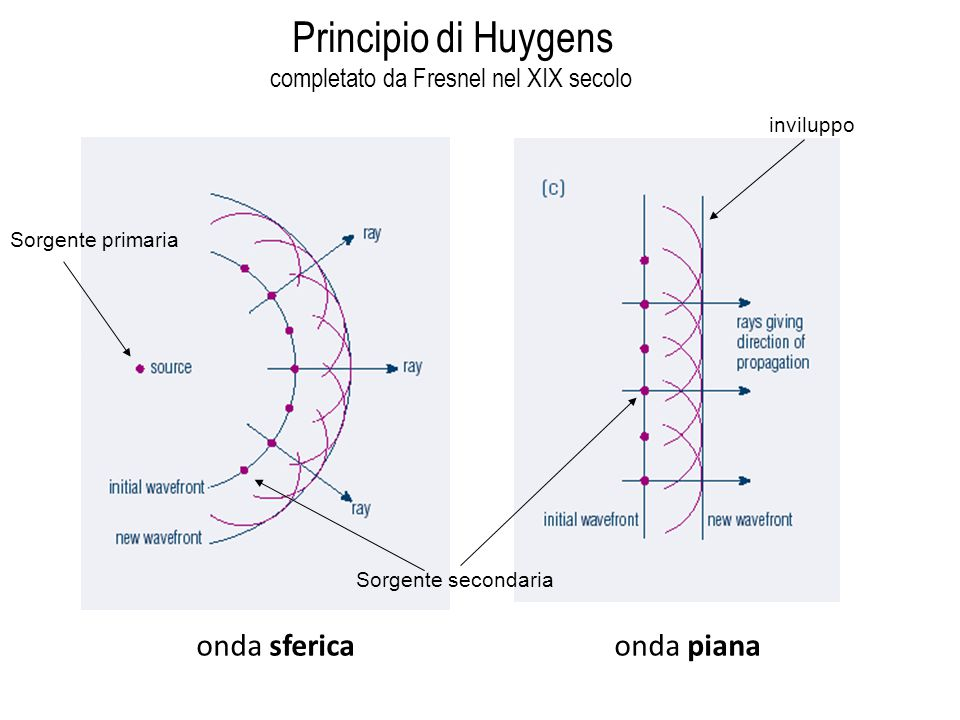
\includegraphics[scale=0.35]{figures/huygens.jpg}
	\caption {Principio di Huygens-Fresnel} 
	\label{fig:huygens}
	\end{figure}

\item \textbf{Principio di Rayleigh}: questo principio riguarda la diffrazione in quanto se un fronte d'onda colpisce una fenditura di dimensioni paragonabili alla sua lunghezza d'onda, esso verrà ritrasmesso al di la della fenditura come se fosse una sorgente puntiforme.

\end{itemize}

Il salto concettuale ora è breve in quanto se una sorgente acustica reale emette un fronte d'onda ed esso impatta in una serie di fenditure disposte spazialmente in un modo preciso, il fronte d'onda passerà al di ognuna delle fenditure (principio di Rayleigh) e la somma della totalità dei fronti d'onda secondari ricreerà esattamente il fronte d'onda originale.

Ora l'unica cosa che è rimasta da fare è sostituire ogni fenditura con un altoparlante e far riprodurre ad esso un  segnale preciso che combinato con i segnali degli altri altoparlanti ricreerà fedelmente (almeno a livello concettuale) lo spazio sonoro che vogliamo ottenere

\begin{figure}[htbp]
	\centering
	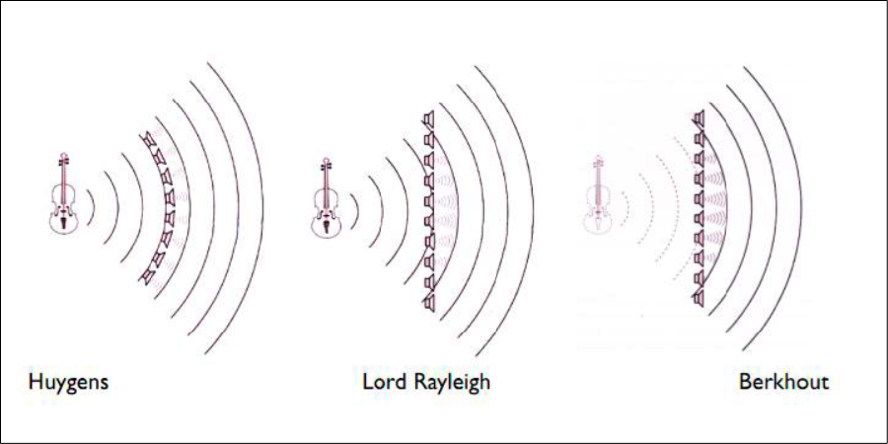
\includegraphics[scale=0.55]{figures/wfs.png}
	\caption {Salti concettuali della WFS} 
	\label{fig:wfs}
	\end{figure}
	

Ora le questioni che ci vengono naturali sono come e con quale segnale pilotare ogni altoparlante; le risposte possono essere molteplici ma tutte devono tener conto della geometria di progettazione del nostro sistema WFS, prendiamo uno dei casi più semplici.\\










\begin{thebibliography}{}


\end{thebibliography}
\addcontentsline{toc} {chapter}{Bibliografia}




\end{document}

